\begin{table}[!htbp]
\centering
\caption{Ablation (5 seeds $\times$ 10 scenes per condition). AUC@5, catastrophic rate (\%), 90\%-bound coverage (\%), inlier edges kept (\%) and outlier edges rejected (\%).}
\label{tab:ablation}
\setlength{\tabcolsep}{2.2pt}
\scriptsize
\resizebox{\columnwidth}{!}{%
\begin{tabular}{lcccccccc}
\toprule
 & Clean & \multicolumn{2}{c}{Fog $2\times$} & \multicolumn{5}{c}{Heavy $3\times$, 35\% outl.}\\
\cmidrule(lr){2-2}\cmidrule(lr){3-4}\cmidrule(lr){5-9}
Variant & AUC@5 & AUC@5 & Cov. & AUC@5 & Cat. & Cov. & Inl.\ kept & Outl.\ rej.\\
\midrule
CARA (full) & 0.815 & 0.642 & 93.1 & 0.387 & 0.32 & 97.3 & 96.9 & 99.2\\
\midrule
no recalibration & 0.790 & 0.594 & 92.6 & 0.303 & 6.86 & 89.5 & 90.4 & 97.1\\
median triangle score & 0.814 & 0.641 & 92.8 & 0.379 & 0.70 & 98.2 & 98.3 & 98.4\\
no rescue round & 0.815 & 0.642 & 93.2 & 0.387 & 0.50 & 97.0 & 96.5 & 98.8\\
no residual gate & 0.814 & 0.641 & 92.6 & 0.381 & 1.90 & 94.6 & 90.4 & 64.9\\
no weight clipping & 0.814 & 0.640 & 92.9 & 0.385 & 0.42 & 97.2 & 96.9 & 99.1\\
connect-back instead of consensus & 0.814 & 0.641 & 93.1 & 0.380 & 2.24 & 95.0 & 94.4 & 98.4\\
no 2-core pruning & 0.814 & 0.641 & 93.1 & 0.381 & 2.02 & 95.3 & 94.7 & 98.5\\
no drift factor & 0.813 & 0.574 & 43.4 & 0.201 & 9.92 & 13.1 & 45.9 & 99.5\\
$\hat\rho_{\mathrm{safe}}$ instead of $\hat\rho_{\mathrm{pt}}$ & 0.817 & 0.644 & 92.4 & 0.181 & 4.08 & 86.5 & 98.0 & 91.8\\
fixed kernel scale & 0.813 & 0.573 & 85.1 & 0.218 & 0.42 & 82.6 & 92.7 & 99.3\\
no final soft refinement & 0.805 & 0.621 & 92.4 & 0.380 & 0.34 & 97.8 & 96.9 & 99.2\\
$\alpha_{\mathrm{edge}}{=}\alpha_{\mathrm{res}}{=}0.05$ & 0.815 & 0.642 & 93.1 & 0.386 & 0.70 & 97.1 & 98.9 & 98.5\\
$\alpha_{\mathrm{edge}}{=}\alpha_{\mathrm{res}}{=}0.20$ & 0.815 & 0.642 & 93.1 & 0.387 & 0.56 & 96.6 & 91.7 & 99.2\\
\bottomrule
\end{tabular}}
\end{table}


\section{Ablation}\label{sec:ablation}
\Cref{tab:ablation} removes one component at a time on five seeds that are separate from the main study (the random streams of a few scenes coincide across conditions and with the main study's seed 0; they differ in noise level and outlier rate). Two components carry most of the gain under shift, and both are tied to the drift factor. Without $\hat\rho$, AUC@5 in the heavy condition drops from $0.387$ to $0.201$, 45.9\% of inlier edges survive, and bound coverage falls to 13.1\%. With $\hat\rho$ but a fixed kernel scale, AUC@5 drops to $0.218$, which is consistent with part (c) of \cref{lem:equiv}: a kernel tuned for clean noise treats inflated inlier residuals as outliers. Recalibration matters most when noise and outliers are both high (AUC@5 $0.303$ and 6.9\% catastrophic without it). The residual gate is what rejects outliers that pass the cycle test: without it, outlier rejection in the heavy condition falls from 99.2\% to 64.9\% and the catastrophic rate rises from 0.32\% to 1.90\%. Replacing consensus bridging by connect-back, or removing 2-core pruning, has almost no effect on AUC but raises the catastrophic rate to 2.24\% and 2.02\%, which is the purpose of those steps. The final soft refinement adds $0.010$--$0.021$ AUC@5 on clean and fog scenes. Weight clipping, the rescue round and the choice of median versus low-quantile aggregation change AUC by at most $0.008$ here; we keep them because they cost nothing and protect against confidently wrong edges and contaminated triangles, but the data do not show that they are needed. The risk levels behave as designed: with $\alpha_{\mathrm{edge}}=\alpha_{\mathrm{res}}=0.05$ CARA keeps 97.9\% of inlier edges on clean scenes and with $0.20$ it keeps 82.5\%, while accuracy barely changes, so $\alpha$ trades inlier retention against nothing measurable in this range.


\clearpage
\begin{figure}[!htbp]
\centering
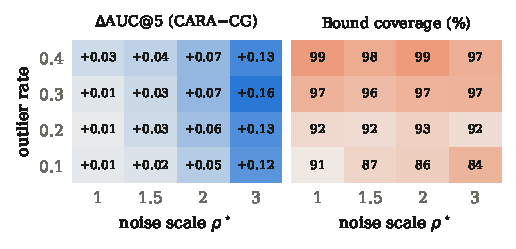
\includegraphics[width=\linewidth]{figs/grid.pdf}
\caption{Robustness grid (3 seeds $\times$ 6 scenes per cell), calibrated at noise scale $1$ and outlier rate $0.2$. Left: AUC@5 gain over CG (blue: CARA better). Right: coverage of 90\% bounds; shading grows with the distance from 90\%.}
\label{fig:grid}
\end{figure}

\section{Robustness grid}\label{sec:grid}
\Cref{fig:grid} varies the noise scale from $1$ to $3$ and the outlier rate from $0.1$ to $0.4$, with calibration fixed at $(1, 0.2)$. CARA has higher mean AUC@5 than CG in all 16 cells (gain $+0.006$ to $+0.157$) and higher than CG-$\hat\rho$ in all 16 (gain $+0.006$ to $+0.042$), and its catastrophic rate is at most that of CG in every cell except one ($1.8\%$ vs.\ $1.7\%$). Coverage depends on the outlier rate as well as on noise: when the test scenes have \emph{fewer} outliers than the calibration scenes (rate $0.1$), coverage under noise shift falls to 84--87\%, and when they have more it rises to 96--99\%. The outlier rate shifts the low quantile of cycle scores that $\hat\rho$ reads, so a change in outlier rate is partly absorbed into the drift factor. This is a second shift dimension that a scalar correction handles only approximately.


\begin{figure}[!htbp]
\centering
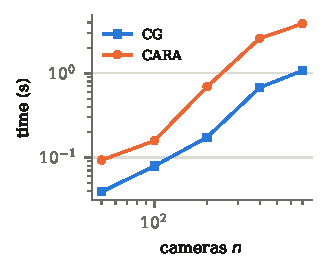
\includegraphics[width=0.55\linewidth]{figs/runtime.pdf}
\caption{Median single-thread runtime per scene (about $5.5$ edges per camera).}
\label{fig:runtime}
\end{figure}

\section{Runtime}\label{sec:runtime}
CARA costs 2--4 times as much as CG on the synthetic graphs in our implementation (\cref{fig:runtime}): $0.16$\,s vs.\ $0.08$\,s at 100 cameras and $3.9$\,s vs.\ $1.1$\,s at 700 cameras. The extra time goes to triangle scoring, the two gated solves and bridging. On the dense 715-camera Notre Dame graph (64,678 edges) the ratio is 6.2 (70\,s against 11\,s). Calibration is a one-time cost per front end and scene type (about 11\,s for 140 synthetic 100-camera scenes in a separate timing run). Triangle scoring and the Laplacian solves are standard sparse operations and would benefit from a compiled implementation.
